%%
%% This is file `sample-manuscript.tex',
%% generated with the docstrip utility.
%%
%% The original source files were:
%%
%% samples.dtx  (with options: `manuscript')
%% 
%% IMPORTANT NOTICE:
%% 
%% For the copyright see the source file.
%% 
%% Any modified versions of this file must be renamed
%% with new filenames distinct from sample-manuscript.tex.
%% 
%% For distribution of the original source see the terms
%% for copying and modification in the file samples.dtx.
%% 
%% This generated file may be distributed as long as the
%% original source files, as listed above, are part of the
%% same distribution. (The sources need not necessarily be
%% in the same archive or directory.)
%%
%% The first command in your LaTeX source must be the \documentclass command.
%%%% Small single column format, used for CIE, CSUR, DTRAP, JACM, JDIQ, JEA, JERIC, JETC, PACMCGIT, TAAS, TACCESS, TACO, TALG, TALLIP (formerly TALIP), TCPS, TDSCI, TEAC, TECS, TELO, THRI, TIIS, TIOT, TISSEC, TIST, TKDD, TMIS, TOCE, TOCHI, TOCL, TOCS, TOCT, TODAES, TODS, TOIS, TOIT, TOMACS, TOMM (formerly TOMCCAP), TOMPECS, TOMS, TOPC, TOPLAS, TOPS, TOS, TOSEM, TOSN, TQC, TRETS, TSAS, TSC, TSLP, TWEB.
% \documentclass[acmsmall]{acmart}

%%%% Large single column format, used for IMWUT, JOCCH, PACMPL, POMACS, TAP, PACMHCI
% \documentclass[acmlarge,screen]{acmart}

%%%% Large double column format, used for TOG
% \documentclass[acmtog, authorversion]{acmart}

%%%% Generic manuscript mode, required for submission
%%%% and peer review
\documentclass[manuscript,screen]{acmart}

%%
%% \BibTeX command to typeset BibTeX logo in the docs
\AtBeginDocument{%
  \providecommand\BibTeX{{%
    \normalfont B\kern-0.5em{\scshape i\kern-0.25em b}\kern-0.8em\TeX}}}

%% Rights management information.  This information is sent to you
%% when you complete the rights form.  These commands have SAMPLE
%% values in them; it is your responsibility as an author to replace
%% the commands and values with those provided to you when you
%% complete the rights form.
%\setcopyright{acmcopyright}
\copyrightyear{2020}
%\acmYear{2020}
%\acmDOI{10.1145/1122445.1122456}

%% These commands are for a PROCEEDINGS abstract or paper.
%\acmConference[Woodstock '18]{Woodstock '18: ACM Symposium on Neural
 % Gaze Detection}{June 03--05, 2018}{Woodstock, NY}
%\acmBooktitle{Woodstock '18: ACM Symposium on Neural Gaze Detection,
 % June 03--05, 2018, Woodstock, NY}
%\acmPrice{15.00}
%\acmISBN{978-1-4503-XXXX-X/18/06}

%%
%% end of the preamble, start of the body of the document source.
\begin{document}

%%
%% The "title" command has an optional parameter,
%% allowing the author to define a "short title" to be used in page headers.
\title{Spatiotemporal-Aware Visualizations in Augmented Reality Piano Teaching Systems}

%%
%% The "author" command and its associated commands are used to define
%% the authors and their affiliations.
%% Of note is the shared affiliation of the first two authors, and the
%% "authornote" and "authornotemark" commands
%% used to denote shared contribution to the research.
\author{Jordan Aiko Deja}
%\authornote{Both authors contributed equally to this research.}
\email{jordan.deja@famnit.upr.si}
\orcid{1234-5678-9012}
\affiliation{%
  \institution{University of Primorska}
  \city{Koper}
  \country{Slovenia}
  \postcode{6000}
}

\author{Matjaž Kljun and Klen Čopič Pucihar}
\affiliation{%
  \institution{Advisors}
  \city{Koper}
  \postcode{6000}}
\email{matjaz.kljun@famnit.upr.si}

%\author{Klen Čopič Pucihar}
%\affiliation{%
%  \institution{University of Primorska}
 % \city{Koper}
  %\country{Slovenia}
  %\postcode{6000}}
%\email{klen.copic@famnit.upr.si}

%%
%% By default, the full list of authors will be used in the page
%% headers. Often, this list is too long, and will overlap
%% other information printed in the page headers. This command allows
%% the author to define a more concise list
%% of authors' names for this purpose.
\renewcommand{\shortauthors}{Deja, et al.}
%%
%% The abstract is a short summary of the work to be presented in the
%% article.
\begin{abstract}
  Spatiotemporal interactions refer to a range of interactive activities that take place in a particular space at a particular time. The spatiotemporal component in extended reality (XR) allows users to interact with or act based on moving digital elements and visualisations within a particular time frame such as pointing to a moving target, button-clicking, or batting a flying baseball. In such scenarios, users only have a dedicated time window to sense (perceive) the movement of digital elements/visualisations, recognise them, decide on the appropriate response and act accordingly in relation to the moving target. The research on XR spatiotemporal interactions has focused on modelling error rates in spatiotemporal pointing, which allowed designers to mitigate and prevent user errors. However, more work is needed to understand XR spatiotemporal interactions in specific contextualised environments such as XR music teaching systems. AR music teaching systems usually rely on visualisations and other similar cues to help novices learn a specific instrument or a musical piece. These studies have not modeled spatiotemporal interaction as well and have not taken into account users' psycho-cognitive responses. This research proposal attempts to understand the role of spatiotemporal interactions in XR music teaching systems for experts and novices focusing mainly on the piano teaching system. User learning habits, instrument playing patterns and cognitive load will be investigated, observed and will be used to build models in order to design spatiotemporal-aware visualisations, which can enhance music learning experience. 
\end{abstract}
%%
%% The code below is generated by the tool at http://dl.acm.org/ccs.cfm.
%% Please copy and paste the code instead of the example below.
%%
\begin{CCSXML}
<ccs2012>
   <concept>
       <concept_id>10003120.10003121.10003126</concept_id>
       <concept_desc>Human-centered computing~HCI theory, concepts and models</concept_desc>
       <concept_significance>500</concept_significance>
       </concept>
   <concept>
       <concept_id>10003120.10003145</concept_id>
       <concept_desc>Human-centered computing~Visualization</concept_desc>
       <concept_significance>100</concept_significance>
       </concept>
 </ccs2012>
\end{CCSXML}
\ccsdesc[500]{Human-centered computing~HCI theory, concepts and models}
\ccsdesc[100]{Human-centered computing~Visualization}
%%
%% Keywords. The author(s) should pick words that accurately describe
%% the work being presented. Separate the keywords with commas.
\keywords{extended reality, spatiotemporal pointing, piano, music teaching ystems}
%%
%% This command processes the author and affiliation and title
%% information and builds the first part of the formatted document.
\maketitle

\section{Introduction}

Our work will focus on investigating spatiotemporal pointing by exploring augmented reality (AR) music teaching systems - specifically a piano teaching system. Spatiotemporal interactions in immersive environments such as virtual, augmented and mixed reality systems (umbrella term for these is extended reality (XR)) refer to a range of user activities that users need to perform in relation to both time and space. Temporal interaction requires users’ actions within a particular time window in response to an event taking place. For example, several recent studies have explored temporal pointing \cite{lee2016modelling} defined as interaction in which users need to provide a discrete input (e.g., button press), with no or negligible spatial aiming demand (the finger is on the button) in a particular time window (usually very short). Spatial interaction requires users to complete an action at a particular place in space. In contrast to temporal pointing, spatial pointing requires users to aim at a fixed or moving target in space while time is not predefined (e.g. just as quickly as possible). As such, spatiotemporal pointing combines these two principles and is referred to as the user action in an immersive environment as a response to a temporarily available digital stimulus. Examples of spatiotemporal interactions include batting a virtual baseball in a XR environment or hitting the right keys at the right time in an XR piano teaching system. In both examples users need to point to a precise location (hitting the ball with a controller representing the virtual bat or pressing the piano key) at the right time. \\

To be able to complete such spatiotemporal pointing \cite{lee2016modelling}, users have an internal time-keeping mechanism to synchronise their movements to an external stimulus according to the WK model \cite{wing1973response}. Additionally, a response-execution stage that allows the user to process input-stimulus and output-actions, is also needed \cite{wing1973timing}. Other studies have focused on (i) investigating and understanding human cognitive load \cite{radu2009augmented}, (ii) improving the accuracy in the rendering of visual elements (which is also referred to as spatial registration \cite{zheng2013general}), and (iii) discovering novel approaches to minimise latency of visualising overlaying digital visualisations \cite{serafin2017considerations}. \\

Innovations in spatiotemporal interactions also directly contribute to computational human-computer interaction (HCI). The concept of computational HCI considers usage of explicit mathematical models of user-system behavior in order to influence, automate and improve the design process of a system. For example, the collected user data can directly feed back into a model, improving the behaviour of the targets of spatiotemporal interaction. Since extended reality environments present an ideal space to investigate spatiotemporal pointing, we push our contributions further by incorporating techniques in computational HCI. Several formative studies have focused on modelling, predicting, and simulating action and reaction in such environments. These studies have contributed to understanding of (1) how objects move and collide in virtual spaces \cite{lee2017boxer}, (2) how users respond to these objects \cite{lee2016modelling} and (3) how we can foster design affordances that improve their performance \cite{rogers2014piano}.\\

Several piano teaching systems have been built with augmented and virtual reality as a medium for innovation by overlaying augmented time-specific visualisations over piano keys to improve music learning experiences \cite{rogers2014piano, sun2018mr, birhanu2017keynvision}. However, cognitive load and user response times have not been observed and taken into account. Moreover, these prototypes were not based on the pre-built spatiotemporal pointing models. Our research will fill this gap by designing spatiotemporal-aware visualisations based on the pre-built models that take user-data into account, which will in our opinion improve AR piano learning experiences. With this project we are conrtibuting the insights on how modeling spoatiotemporal interaction is benefiting piano learning system. In particular, how can spoatiotemporal-aware models and understanding and taking into account the psycho-cognitive load improve the learning process. 

\section{Related Work}
This section will discuss studies on spatial and temporal interactions on screen and in extended reality (XR) environments followed by the section describing piano teaching systems that use AR visualisations. 

\subsection{Studies on modeling spatiotemporal interactions}
Here we present a few studies in temporal and spatiotemporal pointing and error predicting models. 

\begin{figure}[t]
\centering
 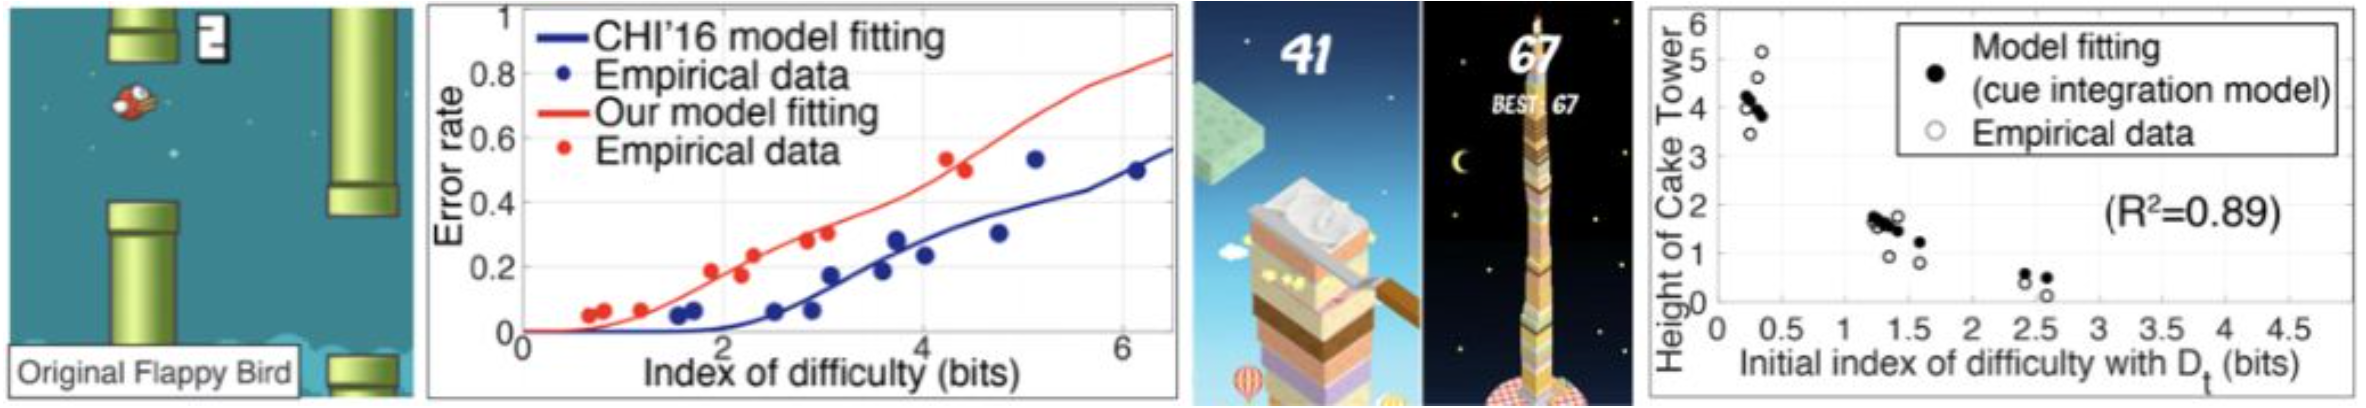
\includegraphics[width=12cm]{figures/flappybird.png}
    \caption{Temporal pointing models could predict player scores and error rates for one-button games such as Flappy Bird (left) and Cake Tower (right).
    }\label{fig:flappybird}
\end{figure}

\begin{itemize}
\item \citet{lee2016modelling} and \citet{lee2018moving} built models to predict players’ performance and error rates in some real-time games that are played with a single button — temporal pointing. Their model could successfully predict the players’ performance while playing popular games such as Flappy Bird and Cake Tower (\ref{fig:flappybird}). The presented model can be applied to adaptively change a game’s difficulty level by changing latency or speed of moving objects). 
\item The study of \citet{lee2017boxer}, investigated collision events of a hand with a virtual object by throwing, pushing or pulling it. In their prototype called Boxer, users received a salient sensory feedback on their palm when a pointer (palm) made a contact with a moving virtual object (a virtual ball). The feedback was triggered when the pointer reached a minimum speed after the collision. The researchers compared this spatiotemporal pointing with a temporal pointing (just pressing a button) presented in the study described before. Based on their findings, spatial precision in collisions improved by 26.7\%. It was also reported that accuracy can be compromised under specific task conditions. Their study also reported that there were no observed differences in temporal precision.
\item The work of \citet{kim2018impact} presented an activation technique called impact activation (IA). This describes the point where a button is activated at its maximal impact point. Based on their findings, IA as a technique is most useful during particularly-rapid repetitive button pressing activities, which are usually observed in games and music applications. While their study focused more on rapid button pressing, their findings were able to report on user’s timing accuracy and how they improved significantly by using IA. The proposed technique can be implemented in modern push-button setups that generate a continuous signal. In music teaching systems, pressing the piano key resembles an action of pressing a button. Users pressing on a setup like a piano teaching system may potentially take advantage from accuracy improvements that use impact activation. 
\end{itemize}

\begin{figure}[t]
\centering
 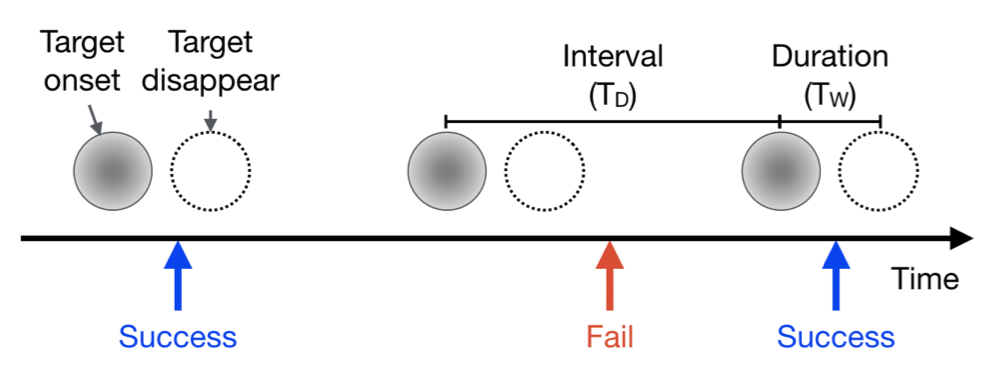
\includegraphics[width=8cm]{figures/boxmodel.png}
    \caption{One of the timing experiments with a box model done by Lee. It considers capturing timing error while the user attempts to catch a target that is regularly blinking.
    }\label{fig:boxmodel}
\end{figure}

Spatiotemporal pointing has been so far mostly investigated outside augmented reality (AR) by modeling, analysing and predicting user error rates. Exploring spatiotemporal pointing in AR is relatively new. The works of \citet{liao2020button, lee2019geometrically, arora2019magicalhands} have laid the groundwork on modeling and measuring spatiotemporal pointing. First by investigating temporal pointing and predicting errors in a task consisting of pressing a button. Recently they explored modelling in XR environments by batting a virtual baseball and authoring animations using gestures in an AR space. Exploration of modeling spatiotemporal pointing in AR music learning is, to the best of our knowledge, nonexistent. Our aim is to expand the presented work by building models for AR music learning and exploring spatiotemporal pointing in these settings. 

\subsection{Studies on music teaching systems, augmented reality and visualizations}

\begin{figure}[h]
\centering
 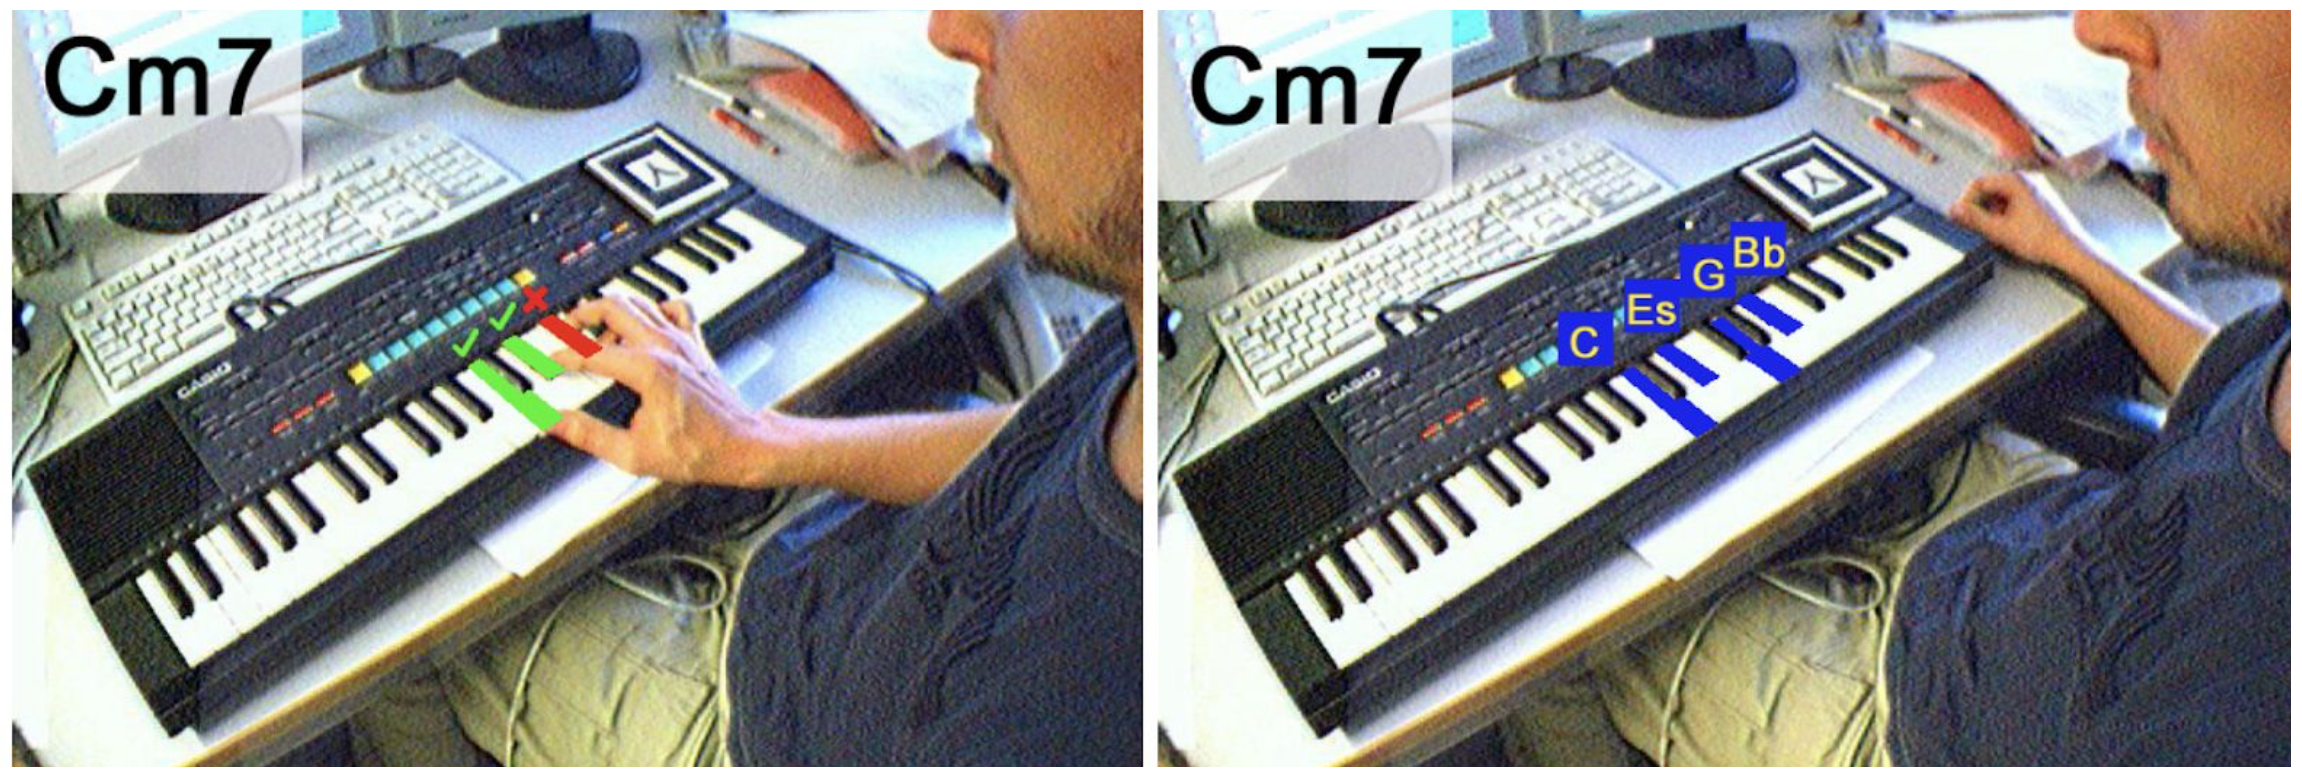
\includegraphics[width=12cm]{figures/barakonyi.png}
    \caption{Prototype by Brakonyi. Visualisations are seen overlying the keys of the MIDI keyboard.
    }\label{fig:barakonyi}
\end{figure}

Computer assisted music teaching systems date back to the early 2000’s. Here we present a couple of examples using XR environments. 

\begin{figure}[h]
\centering
 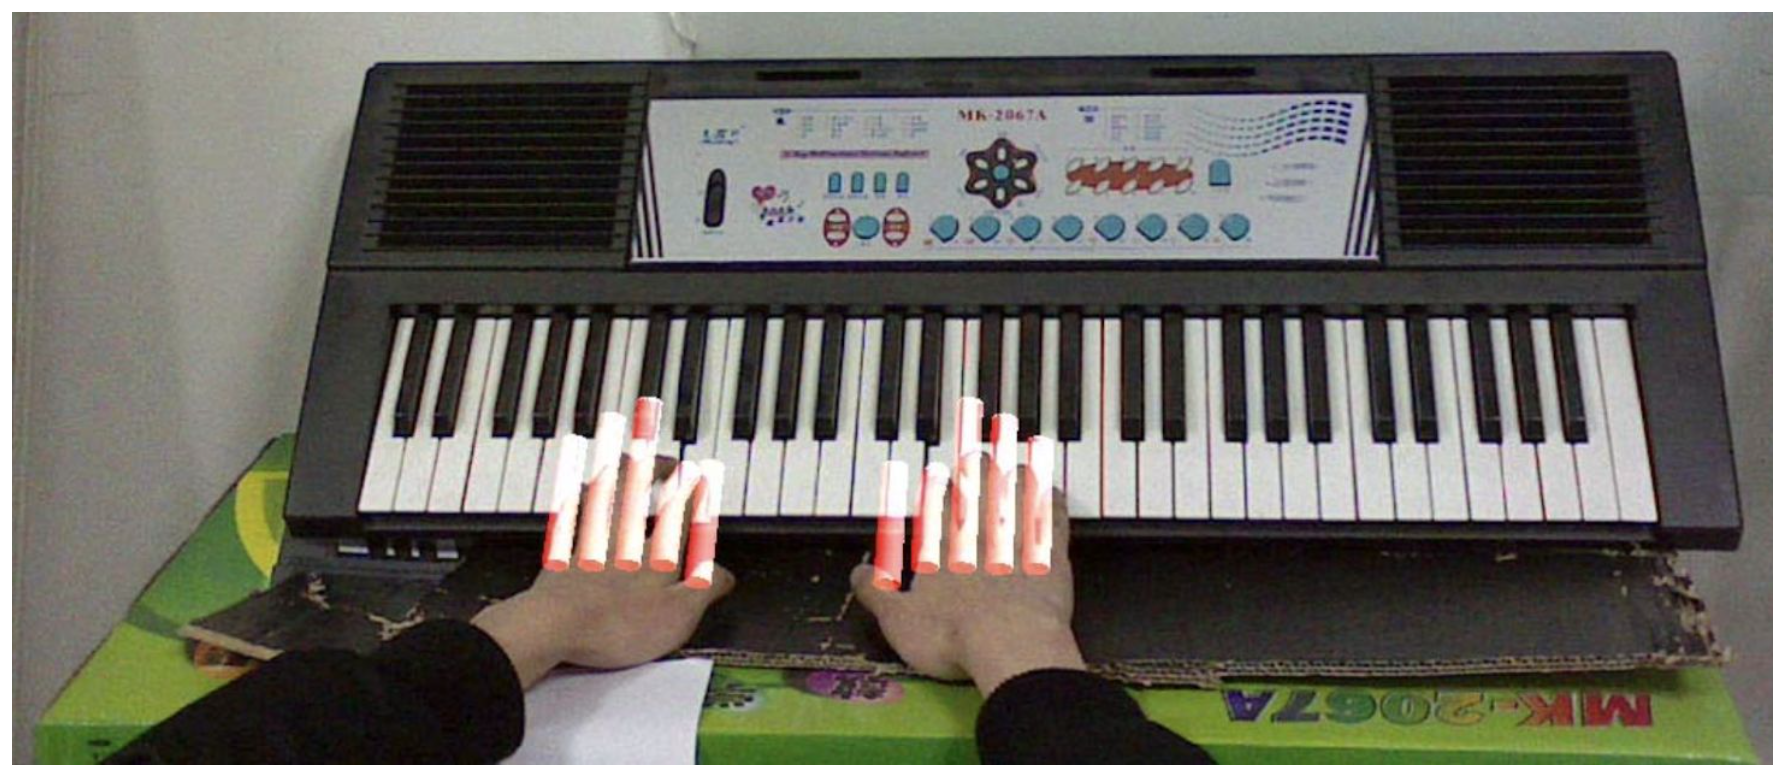
\includegraphics[width=12cm]{figures/huang.png}
    \caption{Prototype by Huang. The virtual hands are seen as overlaid the fingers and keys on the keyboard.
    }\label{fig:huang}
\end{figure}
\begin{figure}[h]
\centering
 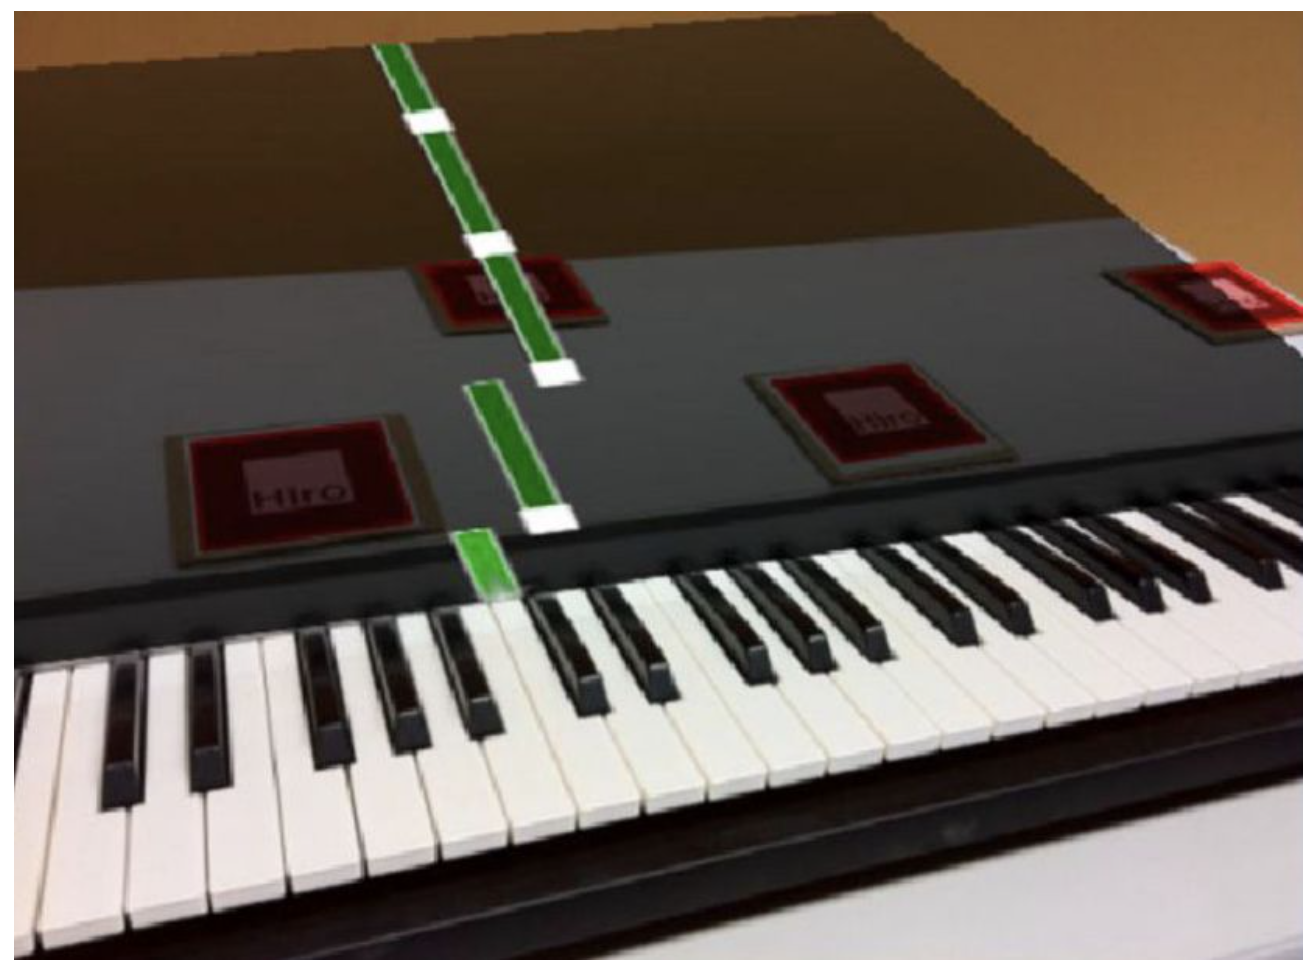
\includegraphics[width=12cm]{figures/chow.png}
    \caption{Prototype by Chow. A piano roll visualisation is seen as “falling notes” in the visualisations.
    }\label{fig:chow}
\end{figure}

\begin{itemize}
\item The work of \citet{barakonyi2005augmented} presented an AR piano tutor seen in Figure \ref{fig:barakonyi}. The prototype used a webcam, a monitor and a MIDI keyboard. The webcam captured the keyboard that was shown on the monitor together with digital information instructing users to hit certain keys in a defined order as well as giving audio feedback as to which keys have been pressed correctly and which were pressed by mistake. The system also included an advanced music composition tool by analysing the tunes currently being played and suggesting background chords and appropriate solo melodies. This technology allows it to understand its users but do not consider other factors such as cognitive load and spatiotemporal pointing data. 
\item The prototype of \citet{huang2011piano} presented a markerless AR based piano teaching system. It used virtual hands overlaid on a real keyboard (Figure \ref{fig:huang}), which allowed the beginners to practice playing the piano. The technology presented in this paper focused on the technological aspects of tracking the real keyboard and overlying virtual hands over the keys. The visualisations used in this prototype did not consider spatiotemporal pointing data. 
\item The paper by \citet{chow2013music} presents an AR prototype using a head mounted display. The prototype is targeting people who practice the instrument on their own (how it is done traditionally) and lack feedback on how to improve their playing as well as motivation for learning. Their prototype addressed these two shortcomings by visualising ``falling'' notes as seen in Figure \ref{fig:chow}} providing direct feedback, and including game elements to learning. The findings show that beginners improved their notation literacy. While the visualisations were effective, we believe that this can be improved further by considering pre-built user models. 
\item The work of \citet{weing2013piano} presents a prototype that enhances musical instrument learning with projected visualisations. Their P.I.A.N.O. prototype (Figure \ref{fig:ubicomp}) aims to support learning to play a piano by considering the learning curve of beginners and addressing hard-to-learn music notations. These notations are replaced by an alternative representation, which are projected onto the piano. Aside from the design of a piano prototype with interactive visualisations and projections, their study also proposed three different learning modes that support novice learners (listen, practice, play modes). They were able to improve on top of the work of \citet{chow2013music} by using gamification and interactivity to prolong student motivation. The P.I.A.N.O. was improved further in \cite{rogers2014piano} by mapping the correct visualisations with extra articulation or enhanced piano roll notation as referred to by authors. Their findings measured (i) significantly lower cognitive load, (ii) improved user experience, and (iii) an increase in perceived music quality rated by the experts as compared against non-projected piano roll notation. 
\end{itemize}
\begin{figure}[h]
\centering
 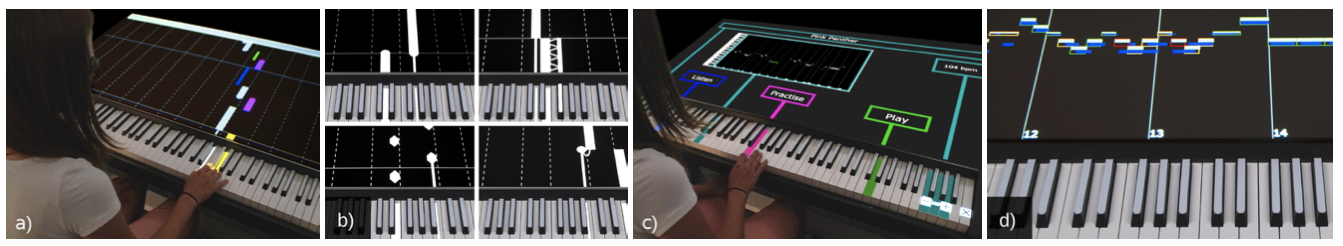
\includegraphics[width=12cm]{figures/pianoUBC.png}
    \caption{Photos of the P.I.A.N.O. interface by Rogers. It included overlaid visualizations, practice modes and detailed feedback. 
    }\label{fig:ubicomp}
\end{figure}

Most of the recent contributions in AR music teaching systems focus on either (1) introducing novel interfaces \cite{barakonyi2005augmented, huang2011piano}, (2) different learner modes for the users \cite{weing2013piano, rogers2014piano}, or (3) improving graphical rendering of the visualisations \cite{chow2013music, zheng2013general}. None of them took users’ cognitive load and response times into account, and were not based on the pre-built spatiotemporal pointing models in order to better support piano learning processes based on users’ performance. Our research will fill this gap by designing spatiotemporal-aware visualisations based on the pre-built models that take user-data into account, which will in our opinion improve AR piano learning experiences.\\

\section{Research Plan and Research Method}
The focus of this research will be on exploring the AR piano teaching system based on the general research question: \textit{“How to  build models based on recording interactions of experts and novices in AR piano teaching systems and use them to design spatiotemporal-aware visualisations that can help novices in their music learning experiences?”}. The models will allow us to understand the differences between the way experts and novices use the developed system while the collected interaction patterns and insights around them will be used to design better visualisations. The elaborated research questions and the research plan are presented in the following subsections. 

\subsection{Research Questions}
Our research is guided by the following research questions: 
\begin{enumerate}
    \item Question: Can we build models of spatiotemporal interactions of expert and novice users while supporting them in playing musical instruments (piano) with AR?  \\
    Hypothesis: We predict that based on the success of earlier studies on spatiotemporal pointing in AR, models of expert and novice usage can also be built for an AR piano teaching system. 
    \item Question: Can we better support learning immersion by considering both spatiotemporal pointing and psycho-cognitive responses of learners while using AR piano teaching systems?\\
    Hypothesis: We believe that if we consider both spatiotemporal pointing and psycho-cognitive responses to visualisation from users when using an AR piano teaching system, we can better support learning immersion.  \citet{lee2016website} states that determining the appropriate level of difficulty in game design is essential to ensure player immersion in a game. By predicting error rates from player’s activities and measuring their psycho-cognitive responses while in game, we could better support player’s immersion. We believe that the same should be true in learning to play musical instruments.
    \item Question: Are there differences in the learning curve and progression of users when using modeled spatiotemporal-aware AR piano teaching systems as compared to using a regular approach? (or standard visualisations?)\\
    Hypothesis: Novices progress differently if they use spatiotemporal-aware modeled visualisations that guide them in a AR piano teaching system. We will measure this by comparing a progress of novices playing a system with and without  spatiotemporal-aware modeled visualisations.
    \item Question: Can the principles and knowledge gained studying the piano spatiotemporal-aware modelled visualisation be adapted to other instruments.\\
    Hypothesis: Music teaching systems that use other instruments (like guitar or xylophone) possess the same elements and conditions required to observe and investigate spatiotemporal pointing. We predict that we can build multi-level (novice, intermediate and expert) models for these systems following the approach we did with the AR piano teaching system. If the later will prove successful we are sure the principles will work for other instruments and provide evidence for the hypothesis. 
\end{enumerate}

\subsection{Method}
This research plan will have six (6) distinct phases. These are:
\begin{itemize}
    \item (Prep-A) Preparation Phase A: Capturing spatiotemporal data from novice and expert users using the AR piano teaching system in order to build two models. 
    \item (Prep-B) Preparation Phase B: Capturing physiological responses from users to understand their cognitive load. 
    \item (Phase-A) Phase A: Designing spatiotemporal-aware visualisations from models of expert and novice users (Prep-A) taking into account also the data captured from physiological responses (Prep-B).
    \item (Phase-B) Phase B: Mitigating user errors in AR piano teaching systems with spatiotemporal-aware visualisations.
    \item (Phase-C) Phase C: Evaluating augmented reality piano teaching systems with spatiotemporal-aware visualisations.
    \item (Phase-D) Phase D: Expanding the process to other instruments such as xylophone, guitar and similar to see it the knowledge can be generalised to other instruments as well. 
\end{itemize}

\begin{table}[H]
\centering
\caption{Gantt Chart. One "\textbullet" represents one month in a quarter. } % removed vspace % add \textbullet ~
\begin{tabular}{|l|l|l|l|l|l|l|l|l|l|l|l|l|}
    \hline
    \multirow{2020-2023} & \multicolumn{2}{|c}{2020}&\multicolumn{4}{|c}{2021}&\multicolumn{4}{|c}{2022}&\multicolumn{2}{|c|}{2023}\\ \cline{2-13} & Q3  & Q4  & Q1  & Q2  & Q3  & Q4  & Q1  & Q2  & Q3  & Q4  & Q1  & Q2  \\ \hline
    Prep-A      & \textbullet\textbullet & \textbullet     &       &       &       &       &       &       &     &     &     &       \\ \hline
    Prep-B      &  & \textbullet\textbullet & \textbullet\textbullet     &       &       &       &       & ~   & ~    &     &     &         \\ \hline
    Phase A     &       &       &       & \textbullet\textbullet\textbullet    & \textbullet\textbullet    &       &       &    &     &     & &  \\ \hline
    Phase B     &       &       &       &       & \textbullet    & \textbullet\textbullet\textbullet     & \textbullet\textbullet     &  &  &  &  & \\ \hline
    Phase C     &       &       &       &       &       &      & \textbullet   & \textbullet\textbullet\textbullet   &    &     &      &     \\ \hline
    Phase D     &       &       &       &       &       &       &       &       &  \textbullet\textbullet\textbullet     & \textbullet\textbullet   & \textbullet\textbullet   &    \textbullet  \\ \hline
\end{tabular}
\label{tab:ganttChart}
\end{table}

In Prep-A we will capture spatiotemporal data from novice and experts while using an AR music teaching system. The data captured will involve specific, primitive activities such as position of fingers on when given a visual stimulus. This data will then be used to build novice and expert models in Phase-A. \\

In Prep-B we will use physiological sensors to collect, measure and understand cognitive load. While phase Prep-A focuses on spatiotemporal pointing data, phase Prep-B focuses on signals related to affect such as Galvanic Sensor Response (GSR), Electrocardiogram (ECG) and others. These multimodal signals will be captured while users perform spatiotemporal pointing activities with the AR piano teaching system. From these setups, we will look at the relationship between hand-eye coordination in key-pressing, heart rate during piano roll, and other rhythm-based synchronisation activities. This phase will help us understand the relationship between (i) cognitive load, the factors that affect them and (ii) spatiotemporal-pointing, and how these two affect the users’ learning curve. \\

The findings from phases Prep-A and Prep-B will be synthesised and used in succeeding phases Phase-A to C. During the Phase-A  we will develop an AR piano teaching systems. While phase Pre-A included spatiotemporal modeling of piano key pressing. Phase-A explores other activities involved in the piano teaching system beyond key-pressing such as, using two hands, chord synchronisation and reading of musical notation all at the same time. Phase-A will at the same time collect physiological sensor data similar to the ones collected from phase Prep-B. From these combined data, we follow the method of Lee et al (2016) in modelling error rates, learner accuracy and precision, reaction times and others. Since this phase will also come up with expert and novice models, we also aim to compare these models and observe differences between these user types. The insights that we will find from these findings will allow us to identify design affordances and other rules that can be used to improve existing visualisations.\\

Phase-B will focus on full development of the prototype using spatiotemporal-aware visualisations, which will consider user data, psycho-cognitive responses and the insights about affordances discovered in previous phases.. The visualisations will give prompt user feedback and the system will adjust based on the pace of its current user to mitigate user errors. This phase will include compatibility tests, expert-novice synchronisation studies, and mixed-method user studies. \\

Phase-C is the summative phase of this research. This phase will involve the design, and evaluation of the developed AR  piano teaching system. This phase will include iterative user evaluations, expert evaluation and other validation activities. This will give us a better understanding with how spatiotemporal pointing aids in improving learning experiences and perceived musical quality similarly as in the cited studies.\\

%Spatiotemporal pointing has been widely-used outside augmented reality. Several studies have done modeling, analysing and predicting error rates. The same set of studies in augmented reality are relatively new and there is much room to explore. Existing HCI work attempts to understand and model human interactions while doing activities with augmented reality music teaching systems.\\

\section{Contributions}
Below are the intended contributions of the research proposed by the author. The research will provide: 
\begin{itemize}
    \item models of spatiotemporal pointing built from the usage data of novices and experts in an AR piano system;
    \item models of cognitive load of novice users in an AR piano teaching system;
    \item guidelines on affordances that improve visualiaations in an AR piano teaching system;
    \item an understanding of how cognitive load and spatiotemporal pointing models can improve the learning experience of novices when learning with an AR piano teaching system;
    \item an augmented reality piano teaching system prototype that considers both cognitive load and spatiotemporal pointing of its users;
    \item an understanding of how the above knowledge can be applied to other AR music teaching system;   
\end{itemize}

\begin{comment}
Most of the recent contributions in augmented reality music teaching systems focus on either (1) introducing a new ubiquitous interface, (2) having different learner modes for the users, and (3) improving graphical rendering of the visualizations. Studies that investigate and model spatiotemporal pointing on augmented reality music teaching systems are very limited. This will be the intended focus of this research. \\
We ask the general research question: “How might we model the interactions of experts and novices when using augmented reality music teaching systems and use them to design spatiotemporal-aware visualizations that can help novices in their music learning experiences?”. We use this general research question as the basis for our hypothesis statements. \\

We will model the spatiotemporal pointing activities of both novices and expert users while using an AR piano teaching systems. We believe that these models will allow us to understand the differences between the way experts and novices use these systems. With this, we will look into their patterns and the insights around them, which in turn we can use to design better visualizations. An overview of the research plan is described in Fig 4. The green branches show a set of experiments that aim to investigate the specific HCI application areas in relation to spatiotemporal pointing and augmented reality music teaching systems (piano, guitar, xylophone, etc). The orange branches show a range of setups that combine results from the experiments done in the green branches, and in relation to sensorimotor and psychophysics, bridging cognitive load and user models. Results of the experiments from the orange and green branches will provide groundwork for this research. The middle branch is the main focus of this thesis. It will focus mainly on augmented reality piano teaching systems. It will investigate the differences between the spatiotemporal models of novices and experts while using these systems. \\
\begin{landscape}
\begin{figure}[h]
\centering
 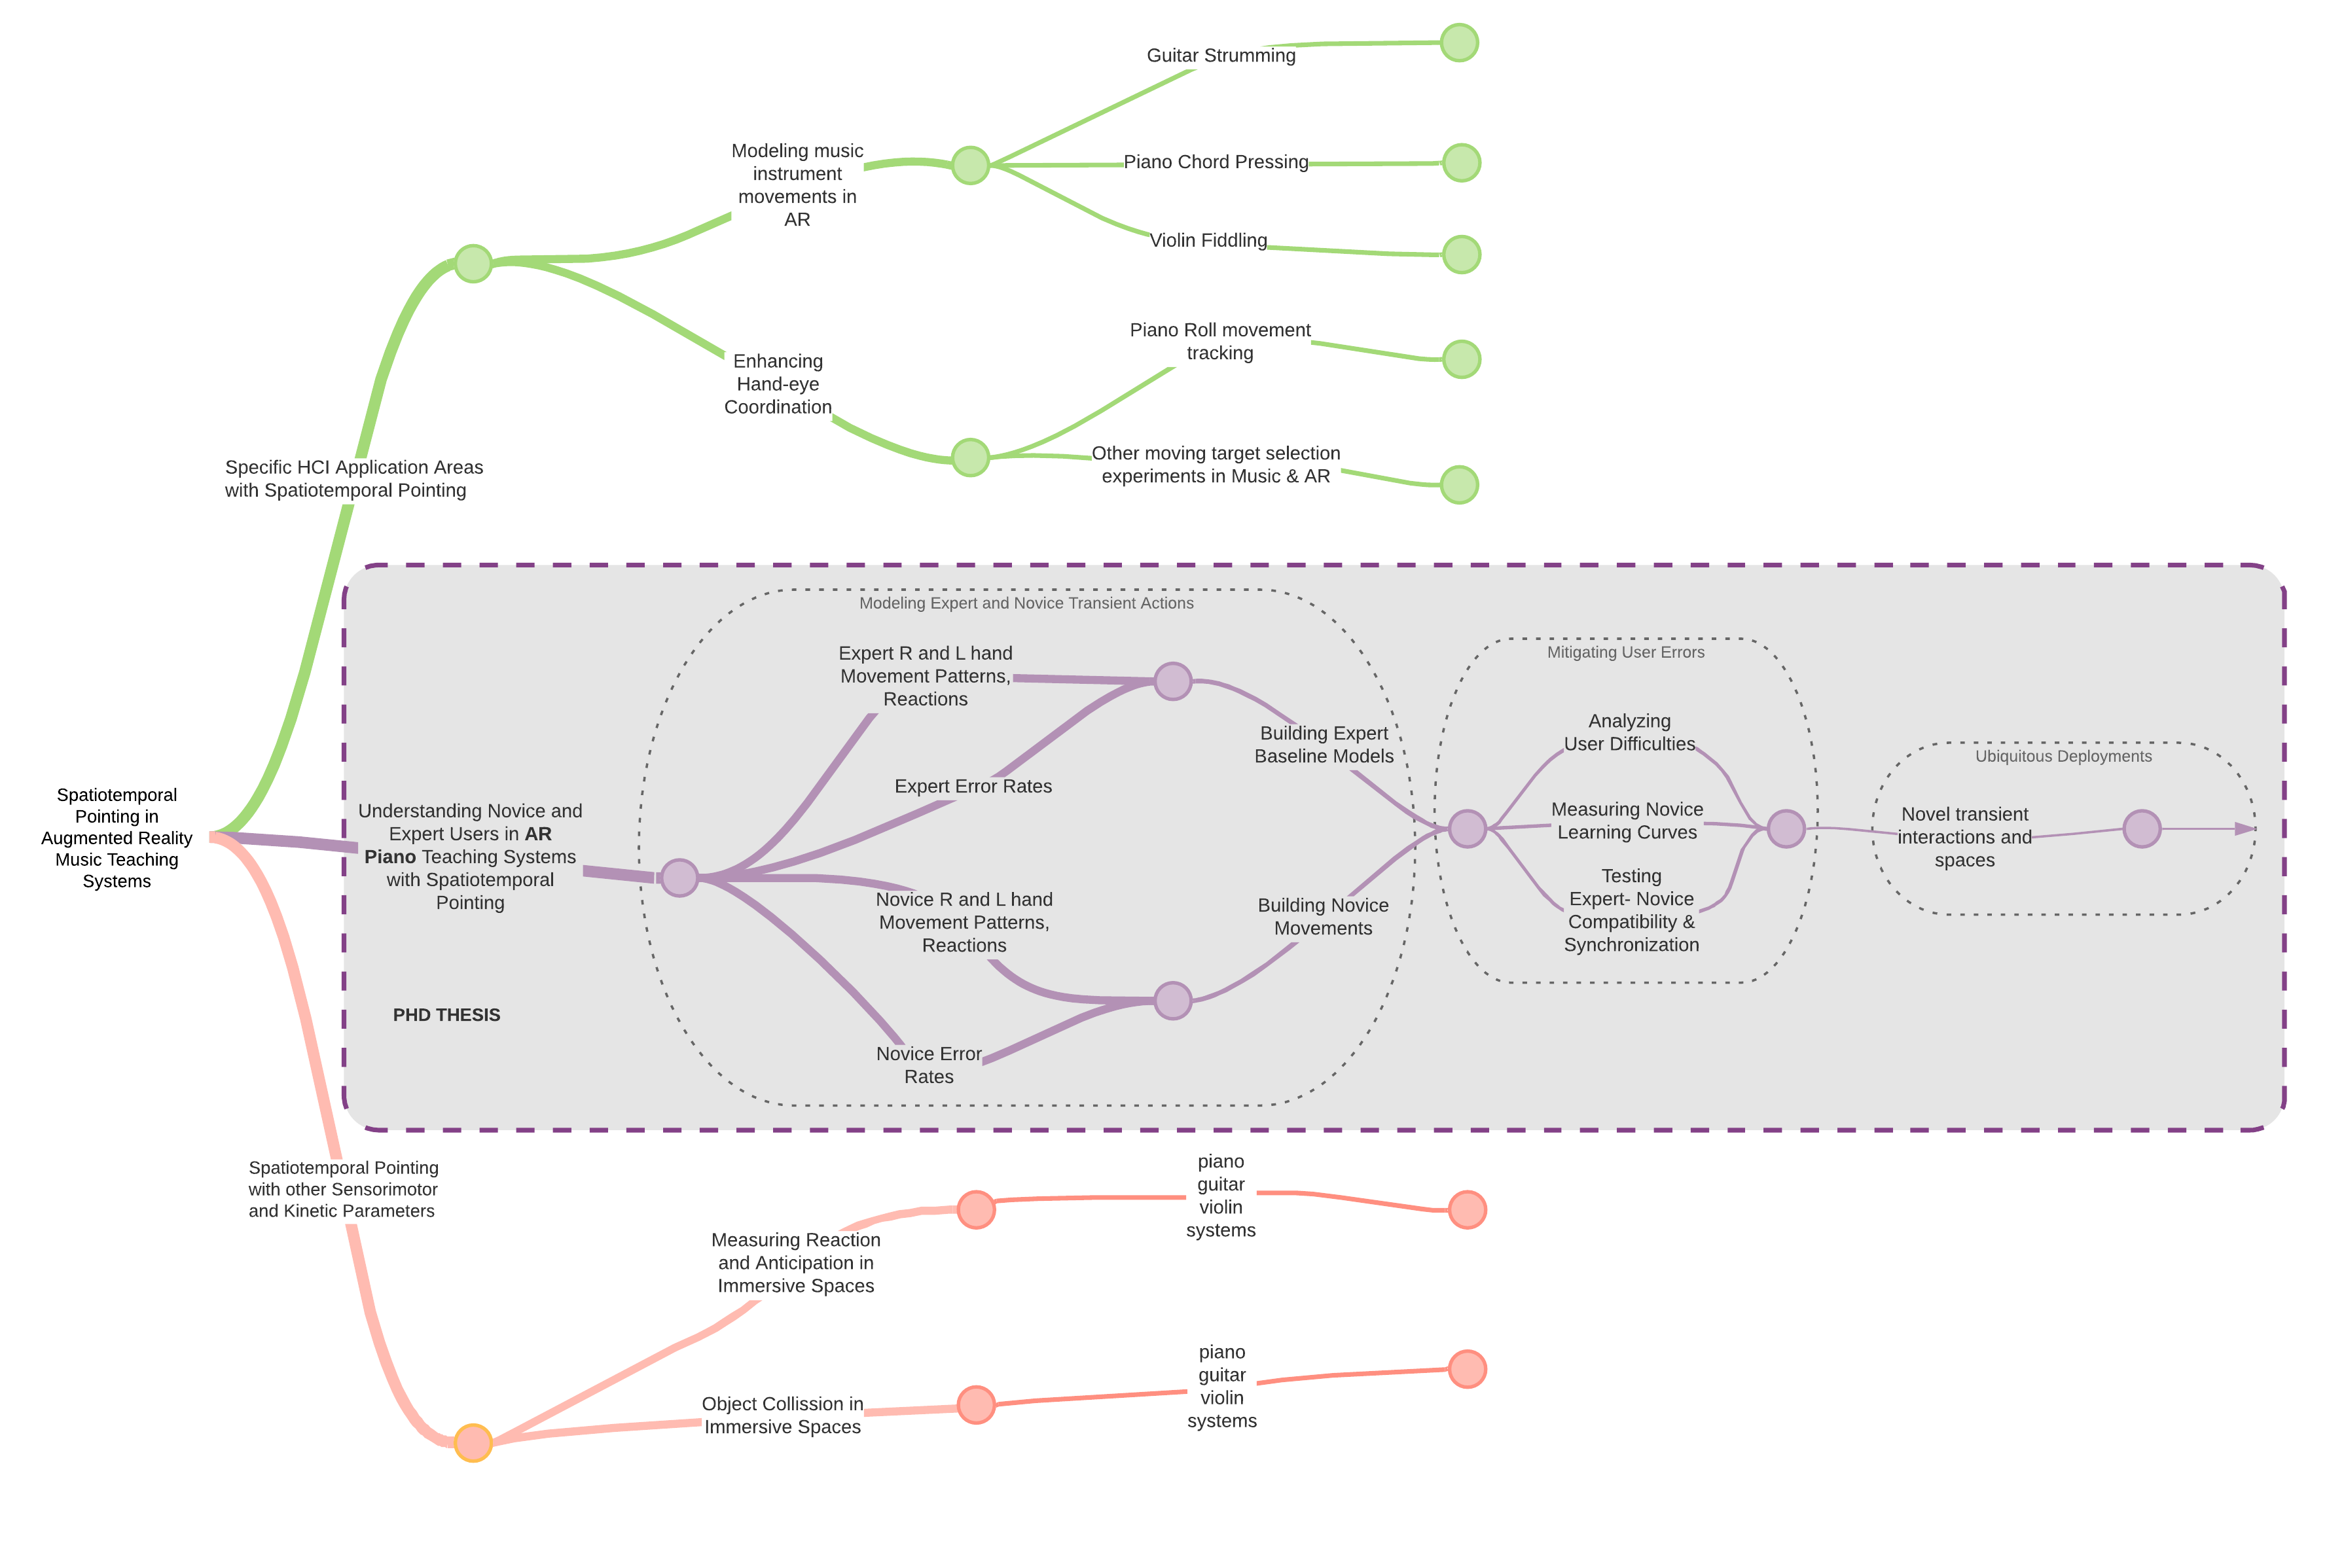
\includegraphics[width=\columnwidth\textheight]{figures/branches.png}
    \caption{An overview of the research branches showing breadth and depth. Each branch represents an experiment which will be part of the methodology in this proposal. Each node in the diagram is targetted  as a concrete contribution leading to a publication.
 }\label{fig:branches}
\end{figure}
\end{landscape}
\end{comment}


%%
%% The next two lines define the bibliography style to be used, and
%% the bibliography file.
\bibliographystyle{ACM-Reference-Format}
\bibliography{sample-base}
%%
%% If your work has an appendix, this is the place to put it.
%\appendix
\end{document}
\endinput
%%
%% End of file `sample-manuscript.tex'.
